\chapter{Basics and state of the art}
\label{sec:state}

% Hier werden zwei wesentliche Aufgaben erledigt:

% 1. Der Leser muß alles beigebracht bekommen, was er zum Verständnis
% der späteren Kapitel braucht. Insbesondere sind in unserem Fach die
% Systemvoraussetzungen zu klären, die man später benutzt. Zulässig ist
% auch, daß man hier auf Tutorials oder Ähnliches verweist, die hier auf
% dem Netz zugänglich sind.

% 2. Es muß klar werden, was anderswo zu diesem Problem gearbeitet
% wird. Insbesondere sollen natürlich die Lücken der anderen klar
% werden. Warum ist die eigene Arbeit, der eigene Ansatz wichtig, um
% hier den Stand der Technik weiterzubringen? Dieses Kapitel wird von
% vielen Lesern übergangen (nicht aber vom Gutachter ;-), auch später
% bei Veröffentlichungen ist "Related Work" eine wichtige Sache.

% Viele Leser stellen dann später fest, daß sie einige der Grundlagen
% doch brauchen und blättern zurück. Deshalb ist es gut,
% Rückwärtsverweise in späteren Kapiteln zu haben, und zwar so, daß man
% die Abschnitte, auf die verwiesen wird, auch für sich lesen
% kann. Diese Kapitel kann relativ lang werden, je größer der Kontext
% der Arbeit, desto länger. Es lohnt sich auch! Den Text kann man unter
% Umständen wiederverwenden, indem man ihn als "Tutorial" zu einem
% Gebiet auch dem Netz zugänglich macht.

% Dadurch gewinnt man manchmal wertvolle Hinweise von Kollegen. Dieses
% Kapitel wird in der Regel zuerst geschrieben und ist das Einfachste
% (oder das Schwerste weil erste).

\section{Virtual Machines and Device Models}
\label{sec:state:virtualization}

Running a guest operating system requires both an execution environment and
access to devices. A virtual machine (VM) provides these resources in the 
form of a virtual computer, while a virtual machine monitor (VMM) is responsible 
for creating and managing this environment.
On Linux, these responsibilities are typically shared between the Kernel-based 
Virtual Machine (KVM) and a userspace VMM. KVM provides hardware-assisted CPU 
and memory virtualization~\cite{kivity2007kvm}, while the userspace VMM manages 
the VM's lifecycle and coordinates access to devices.
QEMU and Cloud Hypervisor are examples of userspace VMMs that use KVM~\cite{johnson2021vfio,cloud-hypervisor}.

In addition to managing the VM's lifecycle, a userspace VMM is responsible for 
providing device access to the guest. This can be achieved through two main approaches: 
\emph{device emulation}, where device behavior is implemented in software, and 
\emph{device passthrough}, where a physical device is assigned to the VM~\cite{bellard2005qfa,santos2008io}. 
In both cases, the guest interacts with devices through their exposed interfaces, 
but the underlying device operations are handled differently.

A separate consideration is where the software responsible for implementing or 
managing a device runs. When a device is supported by a userspace \emph{device model}, 
this software can run either within the VMM process as an \emph{internal device model}, 
or in a separate process that communicates with the VMM as an 
\emph{external device model}~\cite{johnson2021vfio}. In the latter case, migration-relevant 
device state may reside outside the VMM process. Migrating such a VM therefore 
requires coordinating this external state with the rest of the VM state to ensure 
that the guest can resume execution correctly.

\section{Virtual Machine Live Migration}
\label{sec:state:live-migration}

Live migration moves a running VM from a VMM instance to another one while minimizing 
interruptions to the guest machine~\cite{clark2005migration}. In order to ensure that 
execution resumes correctly, the destination must restore a virtual machine state 
that matches the execution state of the source. Therefore, migration must 
coordinate state transitions with the handoff of execution.
To explain this coordination, the section first follows the VM through the
migration lifecycle. It then examines how memory becomes available at the
destination and how device activity remains consistent with that memory.

\subsection{VM State and Migration Lifecycle}
\label{sec:state:migration-lifecycle}

VM migration moves a running VM from one VMM instance, called the \emph{source}, 
to another, called the \emph{destination}. The migration process involves 
preparing the destination, transferring the necessary \emph{VM state}, and coordinating 
the transition of guest execution from the source to the destination~\cite{qemu-migration-framework}.

The VM state consists of three main components: virtual CPU state, guest 
memory, and device state, as illustrated in Figure~\ref{fig:migration-overview}.
CPU state contains the registers and execution context needed to resume 
guest execution, while guest memory holds the data used by the operating 
system and its applications. Device state includes device configuration 
and the status of ongoing I/O operations~\cite{nelson2005migration}. 
For the guest to resume correctly, these components must form a consistent 
state at the destination. For example, information about pending I/O 
requests maintained by a device must be consistent with the corresponding 
data structures in guest memory.

\begin{figure}[htbp]
    \centering
    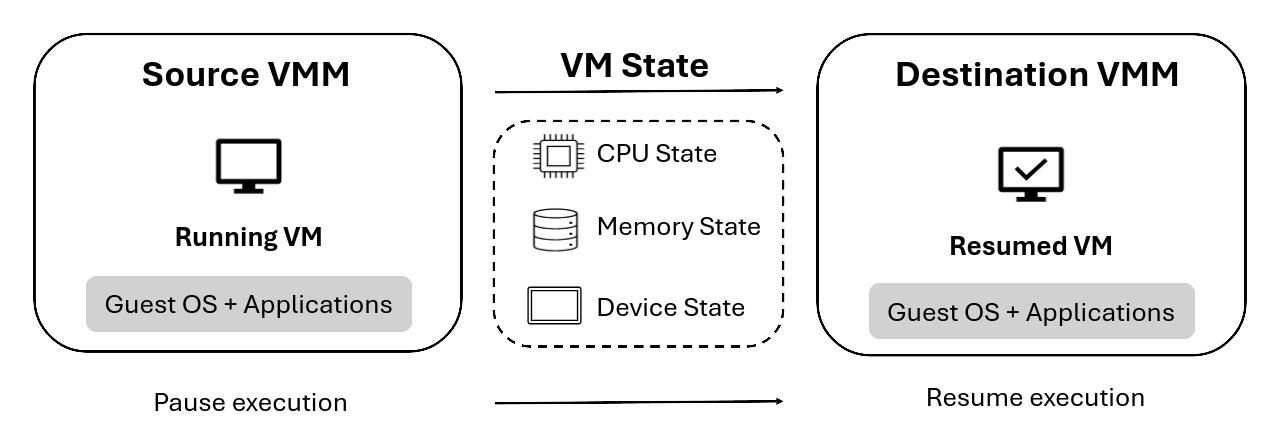
\includegraphics[width=\linewidth]{images/vm-migration.png}
    \caption[VM state and execution handover]{VM migration from a source VMM
    to a destination VMM, preserving CPU, memory, and device state to resume
    the guest.}
    \label{fig:migration-overview}
\end{figure}

Preserving these relationships requires coordination between the source 
and destination throughout the migration process. The destination is 
first prepared with a compatible VM environment and access to the required 
resources. The source and destination then coordinate the transfer of VM 
state and the handover of guest execution. As part of this handover, 
execution stops at the source and resumes at the destination once the 
necessary state has been restored~\cite{nelson2005migration}.

The source and destination VMM instances may run on the same or different 
physical hosts. When both instances run on the same host, this is referred 
to as \emph{same-host migration}; when they run on different hosts, it is 
called \emph{cross-host migration}~\cite{clark2005migration,qemu-cpr}. This 
distinction is particularly relevant to guest memory. In same-host migration, 
the destination may be able to reuse the existing memory backing, whereas 
cross-host migration requires the guest memory to be made available on another machine.

\subsection{Memory Transfer and Resource Reuse}
\label{sec:state:memory-migration}

Another important aspect of VM migration is when guest memory is transferred 
relative to the handover of execution. Two common approaches are \emph{pre-copy} 
and \emph{post-copy} migration~\cite{clark2005migration,hines2009postcopy}.

In \emph{pre-copy} migration, guest memory is copied to the destination 
while the VM continues running on the source. Since the guest may modify 
memory pages that have already been copied, the source tracks these changes 
as \emph{dirty pages} and transfers the modified pages again in subsequent 
rounds. Once the remaining dirty data is sufficiently small, the source 
pauses guest execution and transfers the remaining dirty pages along with 
the final CPU and device state. The destination then restores the VM state 
and resumes guest execution~\cite{clark2005migration}.

In \emph{post-copy} migration, the VM resumes execution at the destination 
before all guest memory has been transferred. The source first pauses guest 
execution and transfers the CPU and device state required for the destination 
to resume the VM. As the guest continues running, accesses to memory pages 
that have not yet been transferred trigger requests to retrieve them from the 
source. Meanwhile, the remaining pages can also be transferred in the 
background~\cite{hines2009postcopy}.

Pre-copy and post-copy primarily describe the timing of memory transfer 
relative to guest execution. A separate consideration is whether guest 
memory must be copied or can be reused at the destination. In cross-host 
migration, the destination typically receives a copy of guest memory because 
the two hosts have separate memory resources. In same-host migration, memory 
can also be copied, but an alternative is to reuse the existing memory 
backing object. This allows the destination to access guest RAM without 
copying its contents. Such reuse requires the backing object to remain 
available and accessible to the destination; running both VMM instances on 
the same host does not automatically provide this access~\cite{clark2005migration,qemu-cpr}.

One way to implement this reuse is to back guest RAM with a file that both 
VMM processes can map into their address spaces. On Linux, an anonymous 
memory-backed file can be created using \emph{memfd}, allowing guest memory 
to be shared without a persistent file on disk~\cite{linux-memfd}. The source 
can pass a file descriptor referring to this backing object to the destination 
through a Unix domain socket~\cite{linux-unix}. The destination can then map 
the same object into its address space, gaining access to the existing guest 
memory without copying its contents. While memory reuse avoids copying guest 
RAM, device state must still be preserved and restored to allow the guest to 
continue its I/O operations correctly.

\subsection{Device State and Migration Consistency}
\label{sec:state:device-migration}

Access to guest memory alone, however, is not sufficient to restore device 
operation. In addition to configuration registers, a device may maintain 
queue positions, pending notifications, and the status of outstanding I/O 
requests. Some of this state is stored outside guest RAM~\cite{qemu-migration-framework,
qemu-vhost-user}. For example, a request buffer in guest memory does not 
indicate whether the device has already processed the request or still needs 
to do so. Without this information, the destination may repeat an already 
completed operation or leave an unfinished one unprocessed.

Ensuring that device operations continue correctly after migration therefore 
involves three key aspects: \emph{state preservation}, \emph{execution 
coordination}, and \emph{device--memory consistency}.

The first aspect, state preservation, requires the destination to 
restore the device state needed to continue operation. Depending on the 
device, outstanding I/O requests may be completed at the source before the 
handover, or their state may be saved and restored so that processing can 
continue at the destination~\cite{qemu-vhost-user}.

The second aspect, execution coordination, concerns when device activity 
is stopped at the source and resumed at the destination. Pausing the virtual 
CPUs alone is not sufficient, as physical devices and I/O workers may continue 
processing requests independently of guest execution. The source must therefore 
quiesce device activity before capturing the final device state, while the 
destination must restore this state before resuming device operations~\cite{qemu-vfio-migration}.

The third aspect, device--memory consistency, concerns how device 
activity affects guest memory during migration. Devices can modify guest 
memory through direct memory access (DMA), independently of virtual CPU 
execution. When memory is copied, a DMA write to an already transferred 
page can leave the destination with outdated data. Such modifications must 
therefore be tracked or otherwise accounted for before the final memory 
state is established~\cite{qemu-vfio-migration}. Although memory reuse avoids 
this problem of outdated copies, device access must still be coordinated with 
the migration handover to maintain consistency between guest memory and device state.

How these requirements are met also depends on where device state and I/O 
processing are managed. For an internal device model, the VMM can coordinate 
device activity and state save/restore operations through its own migration 
framework~\cite{qemu-migration-framework}. With an external backend, however, 
part of the device state and I/O processing resides in a separate 
process~\cite{qemu-multiprocess,qemu-vhost-user}. Saving the VMM's state alone 
is therefore insufficient, as migration must also coordinate backend activity 
and preserve the state maintained outside the VMM. This coordination is necessary 
whether the destination reuses an existing backend or restores device state in a 
separate backend.

\section{VFIO and vfio-user for External Device Models}
\label{sec:state:vfio-user}

When a device model runs outside the VMM, the VMM must communicate with it 
during both normal operation and migration. vfio-user supports this interaction 
through a userspace client--server protocol that builds on concepts from Linux 
VFIO. This section introduces the relationship between VFIO and vfio-user, 
explains how the VMM interacts with an external device backend, and examines 
the protocol mechanisms for device migration.

\subsection{From VFIO to vfio-user}
\label{sec:state:vfio-interface}

Device passthrough requires a userspace VMM to configure and manage access 
to physical hardware. On Linux, Virtual Function I/O (VFIO) provides a kernel 
interface for this purpose. Through VFIO, the VMM can access device regions, 
configure interrupts, and establish DMA mappings that allow the device to 
access guest memory. The kernel uses mechanisms such as the I/O memory 
management unit (IOMMU) to restrict device access to permitted memory 
regions~\cite{linux-vfio}.

vfio-user adapts this device-access model to devices implemented in a 
separate userspace process. Instead of interacting with a device through 
the kernel VFIO interface, the VMM communicates with a vfio-user server over 
a socket. The protocol retains VFIO concepts such as device regions, interrupts, 
and DMA access, while the server implements the device's behavior and maintains 
its internal state~\cite{johnson2021vfio}. Since vfio-user does not require a 
physical VFIO device, the server can also implement a virtual device entirely 
in software~\cite{libvfio-user-overview}. This separation allows the VMM to 
provide device access to the guest while the device implementation resides in 
an external backend.

\subsection{Client--Server Architecture and Device Operation}
\label{sec:state:vfio-user-architecture}

The separation between the VMM and the device implementation in vfio-user
follows a client--server architecture, as illustrated in
Figure~\ref{fig:vfio-user-architecture}. The VMM acts as the \emph{client},
while the external backend combines a vfio-user \emph{server} with the
device model. The server handles protocol communication, while the device
model implements device behavior. After establishing a connection over a
UNIX domain socket, the client negotiates the protocol version and
capabilities, then queries the device's PCI regions and interrupt
capabilities. The VMM uses this information to present the device to the
guest~\cite{johnson2021vfio,vfio-user-spec}.

\begin{figure}[htbp]
    \centering
    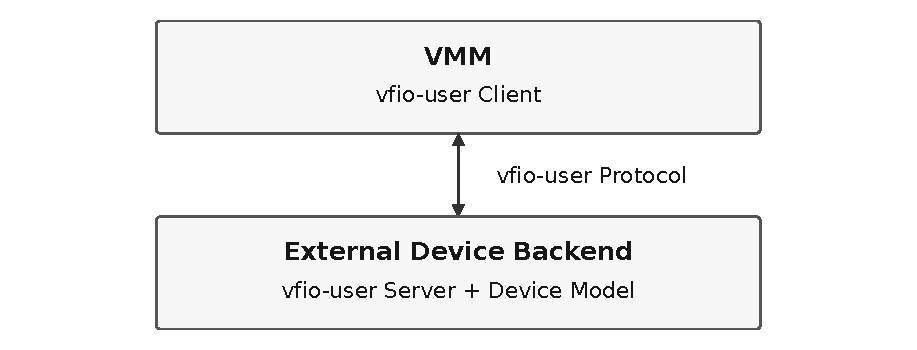
\includegraphics[width=0.85\linewidth]{images/vfio-user-architecture.pdf}
    \caption[vfio-user client--server architecture]{The VMM acts as the
    vfio-user client, while the external device backend implements the
    server and device model.}
    \label{fig:vfio-user-architecture}
\end{figure}

Once the guest begins using the device, the client forwards accesses that 
require device model processing to the server. These accesses may initiate 
I/O requests, for which the backend needs to read request descriptors and 
exchange data with guest memory. To enable this access, the client provides 
the server with information about the memory regions available for DMA and, 
where supported, file descriptors that allow the backend to map these regions 
directly. Alternatively, the backend can access guest memory through vfio-user 
protocol messages. After completing a request, the backend can notify the guest 
through interrupts configured by the client~\cite{vfio-user-spec,libvfio-user-memory}.

Handling these requests involves more than accessing their descriptors and 
data buffers in guest memory. As the device model processes I/O, it may also 
maintain register values, queue positions, and the progress of outstanding 
requests within the backend process~\cite{qemu-multiprocess,hajnoczi2021device-migration}. 
This state is not automatically preserved when the VMM saves its own state 
and guest memory during migration.

\subsection{Protocol Support for Device Migration}
\label{sec:state:vfio-user-migration}

To support migration of an externally implemented device, vfio-user provides 
three mechanisms: migration state control, device-state transfer, and DMA 
dirty logging.

Migration state control allows the client to coordinate device activity with 
the migration process. The client first queries the server's migration 
capabilities, which depend on the device implementation. It then requests 
state transitions through \texttt{VFIO\_USER\_DEVICE\_FEATURE}, using the 
\texttt{VFIO\_DEVICE\_FEATURE\_MIG\_DEVICE\_STATE} feature. A successful reply 
confirms that the server has completed the requested transition, allowing 
the VMM to proceed with the device in the requested state. Table~\ref{tab:vfio-user-migration-states} 
summarizes the main states and their roles during migration
~\cite{vfio-user-spec,linux-vfio-uapi}.

\begin{table}[htbp]
    \centering
    \begin{tabular}{@{}lp{0.67\linewidth}@{}}
        \toprule
        \textbf{State} & \textbf{Role during migration} \\
        \midrule
        \texttt{RUNNING} & The device operates normally. \\
        \texttt{STOP} & Device execution stops and its state no longer advances. \\
        \texttt{STOP\_COPY} & The device remains stopped while exporting its state. \\
        \texttt{RESUMING} & The device loads incoming state without resuming execution. \\
        \texttt{PRE\_COPY} & The device can export state while continuing to operate. \\
        \bottomrule
    \end{tabular}
    \caption[vfio-user device migration states]{Device migration states used
    by vfio-user. \texttt{PRE\_COPY} requires advertised device support.}
    \label{tab:vfio-user-migration-states}
\end{table}

These states also determine when device-state transfer can take place. A 
source backend may export its internal state while operating in the optional 
\texttt{PRE\_COPY} state, but it must stop device execution before exporting 
its final state in \texttt{STOP\_COPY}. At the destination, the backend imports 
the state in \texttt{RESUMING} and returns to \texttt{STOP} before the client 
allows it to enter \texttt{RUNNING}, as illustrated in steps~2--4 of
Figure~\ref{fig:vfio-user-migration-sequence}~\cite{linux-vfio-uapi}.

In step~3 of Figure~\ref{fig:vfio-user-migration-sequence}, the source
client reads the device state through \texttt{VFIO\_USER\_MIG\_DATA\_READ}. 
The source VMM transfers this data to the destination VMM, which supplies 
it to the destination backend through \texttt{VFIO\_USER\_MIG\_DATA\_WRITE}. 
The backend determines how to save and restore its device-specific state, 
while the VMM coordinates the transfer between source and destination~\cite{vfio-user-spec}.

Beyond preserving device state, migration must also account for changes that 
the backend makes to guest memory through DMA. In particular, writes through 
shared memory mappings may not be captured by the VMM's tracking of virtual 
CPU writes. The client can separately query whether the server supports DMA 
dirty logging and, when available, enable logging and retrieve bitmaps of
pages modified by DMA. Steps~1 and~2 of
Figure~\ref{fig:vfio-user-migration-sequence} show logging setup and a final
bitmap query after the device stops. The VMM can incorporate these pages into memory pre-copy 
alongside pages modified by the virtual CPUs. Before completing the handover, 
it must also account for device writes up to the point where device activity 
stops, ensuring that the destination receives a consistent memory state~\cite{vfio-user-spec,qemu-vfio-migration}.

Figure~\ref{fig:vfio-user-migration-sequence} illustrates how these
device-level operations fit into the overall VM migration process.
Although vfio-user provides interfaces for migration state control,
device-state transfer, and DMA dirty logging, the VMM determines how
to integrate these mechanisms with CPU execution, guest-memory handling,
and destination resumption. This integration depends on the VMM's
migration architecture and how it coordinates external device backends.

\begin{figure}[htbp]
    \centering
    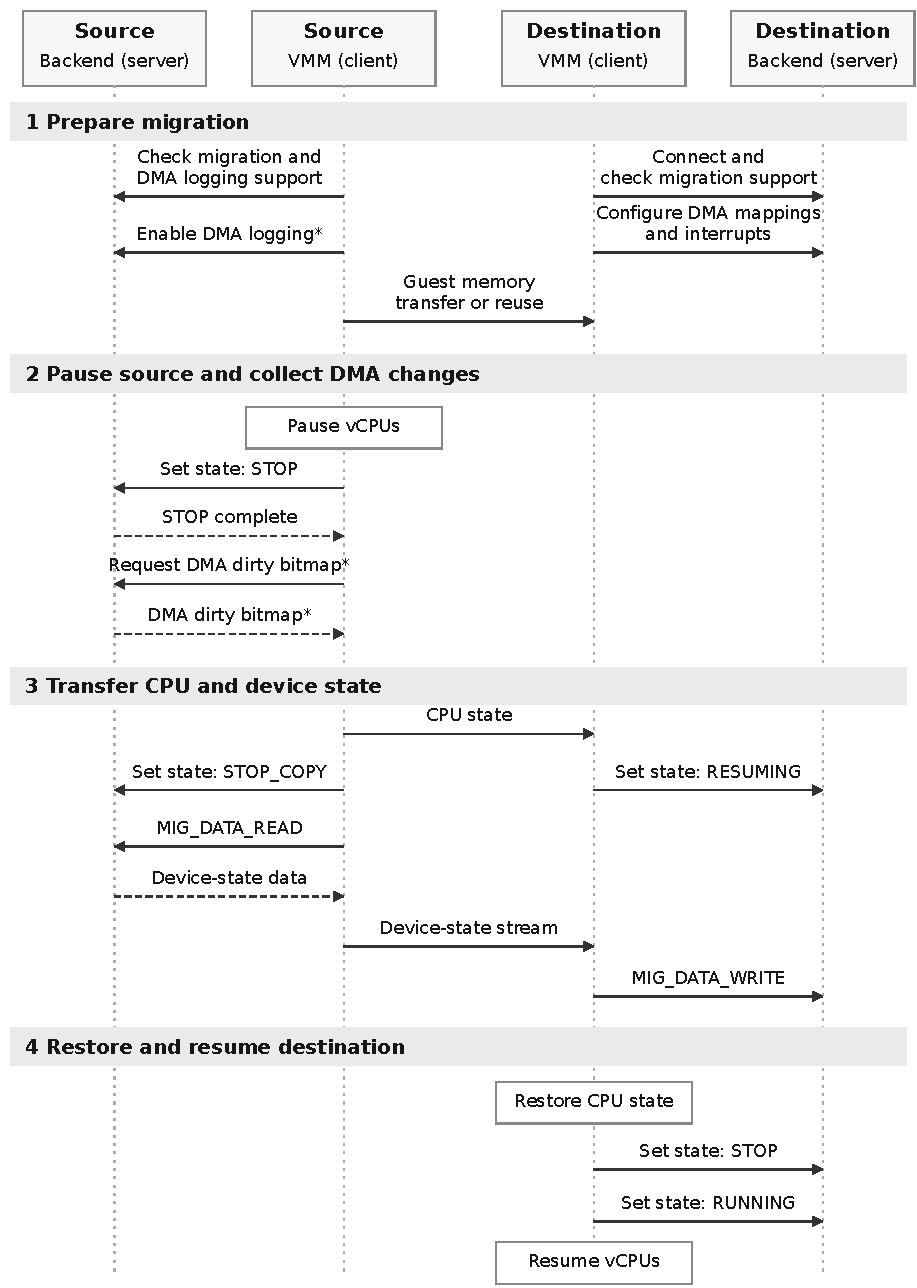
\includegraphics[width=\linewidth]{images/vfio-user-migration-sequence.pdf}
    \caption[VM migration with vfio-user]{VM migration with a vfio-user device, 
    showing a simplified stop-and-copy sequence. Boxes indicate local VMM actions, 
    dashed arrows represent selected replies, and asterisks mark optional DMA dirty 
    logging. Device-state read and write operations may repeat until the transfer 
    is complete. Guest-memory handling is shown schematically and may involve memory 
    transfer or reuse, depending on the migration method.}
    \label{fig:vfio-user-migration-sequence}
\end{figure}

\section{Migration Support in Existing VMMs}
\label{sec:state:vmm-migration}

The migration mechanisms introduced in the previous sections require 
integration into a VMM's migration framework to coordinate device state 
with the rest of the VM. This section examines how QEMU and Cloud 
Hypervisor implement this integration, focusing on their existing 
migration capabilities and support for external devices.

\subsection{Migration Infrastructure in QEMU}
\label{sec:state:qemu-migration}

QEMU provides a concrete example of how a VMM incorporates device state
into VM migration. For device models implemented within its own process,
QEMU directly manages their internal state. For example, its emulated
xHCI USB controller maintains controller registers and runtime state
inside the VMM~\cite{qemu-xhci-migration}. Restoring this controller at
the destination requires preserving the state needed to continue its
operation. Migratable device models typically identify this state
through a versioned \texttt{VMStateDescription}, which specifies the
fields to serialize and may include callbacks for additional processing
during save and restore. The migration framework uses these descriptions
to save device state into the VM migration stream and restore it at the
destination~\cite{qemu-migration-framework}.

For physical devices assigned through VFIO, QEMU relies on the host
device's VFIO driver to expose the internal state required for migration.
It accesses this state through the kernel VFIO migration interface and
registers save and load handlers with its migration framework. These
handlers transfer device state, while VM run-state handlers coordinate
device execution with the migration lifecycle. During the final handover,
QEMU stops the device and exports its remaining state, which the
destination loads before resuming device execution. During memory migration, 
VFIO devices may continue modifying guest memory through DMA while QEMU 
transfers its contents. QEMU therefore uses VFIO dirty-page reporting to 
track these changes and ensure that the destination receives the updated 
memory pages~\cite{qemu-vfio-migration}.

A similar challenge arises with vfio-user devices, where a separate
userspace backend maintains the device state rather than exposing
physical-device state through a kernel VFIO driver. QEMU's existing VFIO
migration infrastructure therefore provides a basis for integrating these
devices into the VM migration lifecycle. A patch series proposed by
Komatsu in September 2026 follows this approach by extending the existing
\texttt{VFIODeviceIOOps} abstraction to cover migration operations.
The vfio-user frontend supplies socket-based implementations of these
operations, allowing it to reuse QEMU's VFIO migration handlers.
The series also integrates DMA dirty logging and registers vfio-user
PCI devices with the migration framework. In the v2 series, device-state
transfer uses stop-and-copy; the implementation does not enable
device-state pre-copy or peer-to-peer migration states
~\cite{komatsu2026vfio-user-migration}.

Besides preserving device state, migration also requires the destination 
to obtain access to the resources on which the VM depends. When both VMM 
instances run on the same host, some of these resources can remain in 
place rather than being copied or recreated. QEMU supports this approach 
through its \emph{CheckPoint and Restart} (CPR) mechanism. In 
\texttt{cpr-transfer} mode, a replacement QEMU process takes over the VM 
while retaining its existing shared memory backing. QEMU transfers VM 
state through the migration channel and passes file descriptors for 
retained resources through a separate UNIX domain socket. This allows 
the replacement process to reuse guest RAM without copying its contents 
and, for supported VFIO and IOMMUFD configurations, preserve device 
resources and pinned memory pages across the handover~\cite{qemu-cpr}.

\subsection{Migration Support in Cloud Hypervisor}
\label{sec:state:cloud-hypervisor-migration}

Cloud Hypervisor provides mechanisms for migrating guest memory and restoring 
VM component state. The following examine its memory migration capabilities, 
particularly same-host memory reuse, and its support for device migration.

\subsubsection{VM Migration in Cloud Hypervisor}
\label{sec:state:cloud-hypervisor-vm-migration}

Cloud Hypervisor is a Rust-based VMM designed for cloud workloads, with an 
emphasis on minimal hardware emulation and support for virtio and passthrough 
devices~\cite{cloud-hypervisor}. Its migration framework coordinates the 
transfer of guest memory with the restoration of CPU and device state. For 
guest memory, Cloud Hypervisor supports three migration modes: \texttt{precopy}, 
\texttt{postcopy}, and \texttt{memfds}. The first two implement the 
memory-transfer strategies introduced in Section~\ref{sec:state:memory-migration}, 
while the third applies the resource-reuse approach for migration between VMM 
processes on the same host~\cite{cloud-hypervisor-live-migration}.

Similar to QEMU's \texttt{cpr-transfer}, Cloud Hypervisor's \texttt{memfds} 
mode allows the destination to reuse existing guest-memory backing rather than 
copying its contents. Cloud Hypervisor implements this by passing the backing 
file descriptors over a UNIX domain socket. This requires shareable memory 
backing, such as shared memory or suitable hugepage backing. The source sends 
the descriptors together with information identifying their corresponding 
memory regions, allowing the destination to map the same backing into its own 
address space~\cite{cloud-hypervisor-live-migration,cloud-hypervisor-migration-code,cloud-hypervisor-memory-code}. 
Since both VMM instances access the same underlying memory, this mode does not 
require iterative RAM copying or the dirty-page tracking associated with it. 
However, reusing guest memory does not eliminate the need to transfer CPU and 
device state, which Cloud Hypervisor must still restore before the destination 
resumes execution.

\subsubsection{Device Migration in Cloud Hypervisor}
\label{sec:state:cloud-hypervisor-device-migration}

Cloud Hypervisor manages device state through its component migration framework. 
Migratable components provide interfaces for pausing and resuming execution and 
capturing their internal state, which the destination uses to reconstruct the 
components. During migration, the framework collects component snapshots into 
a hierarchical representation of the VM. For supported virtual devices, 
including virtio devices, these interfaces allow their state to participate in 
the VM migration process~\cite{cloud-hypervisor-migration-framework}.

For physical devices assigned through kernel VFIO, however, Cloud Hypervisor 
must obtain the device state from the host driver rather than an internal device 
model. It integrates the \emph{VFIO Migration v2 interface} into its component 
migration framework to support devices whose drivers provide migration 
capabilities. When the VM pauses, Cloud Hypervisor stops device execution and 
captures its state through \texttt{STOP\_COPY}. The destination restores this 
state through \texttt{RESUMING} and reestablishes the necessary PCI 
configuration and interrupt settings before device execution resumes. When 
guest memory is transferred using pre-copy, VFIO devices may continue modifying 
it through DMA. Cloud Hypervisor therefore incorporates VFIO dirty-page 
reporting into memory migration to track these changes and ensure that the 
destination receives the updated pages~\cite{cloud-hypervisor-vfio-migration}.

The kernel VFIO integration demonstrates how Cloud Hypervisor can coordinate 
migration for devices whose internal state resides outside the VMM. Cloud 
Hypervisor also supports vfio-user devices during normal VM execution, but 
these devices maintain their state in separate userspace backends rather than 
exposing it through the kernel VFIO interface~\cite{cloud-hypervisor-vfio-user}. 
Migrating them therefore requires the VMM to coordinate backend execution and 
transfer backend state through the vfio-user connection. In the examined 
implementation, however, the vfio-user frontend only snapshots common VMM-side 
PCI state. Its migration lifecycle operations do not control the external 
backend, and the client does not perform the migration-state transitions or 
state transfers needed to preserve its internal state~\cite{cloud-hypervisor-vfio-user-code,cloud-hypervisor-migration-framework}.

As a result, restoring the frontend snapshot alone cannot reconstruct the 
complete device state, even when \texttt{memfds} allows the destination to 
reuse the existing guest RAM. For migration modes that copy memory while the 
device continues performing DMA, Cloud Hypervisor must also account for the 
backend's writes to guest memory. Unlike the kernel VFIO path, the examined 
vfio-user implementation does not yet integrate DMA dirty logging into memory 
migration~\cite{cloud-hypervisor-vfio-user-code}. Supporting these operations 
depends not only on Cloud Hypervisor's migration framework but also on the 
capabilities exposed by the vfio-user client libraries and device backends. 
The following section examines the existing migration support in these components.

\cleardoublepage

%%% Local Variables:
%%% TeX-master: "diplom"
%%% End:
